\chapter{Fundamentação Teórica}
\label{cap:fundamentacao-teorica}

Integer non \textit{lacinia magna}. Aenean tempor lorem tellus, non sodales nisl commodo ut. Proin mattis placerat risus sit amet laoreet. Praesent sapien arcu, maximus ac fringilla efficitur, vulputate faucibus sem. Donec aliquet velit eros, sit amet elementum dolor pharetra eget. Integer eget mattis libero

\section{Fundamentação Teórica A}
\label{sec:fundamentacao-teorica-a}

Integer non \textit{lacinia magna}. Aenean tempor lorem tellus, non sodales nisl commodo ut. Proin mattis placerat risus sit amet laoreet. Praesent sapien arcu, maximus ac fringilla efficitur, vulputate faucibus sem. Donec aliquet velit eros, sit amet elementum dolor pharetra eget. Integer eget mattis libero na \cite{johnsen2005peer}.

	\begin{figure}[h!]
		\centering
		\Caption{\label{fig:bittorrent-2} Arquivo sendo distribuído utilizando  BitTorrent}
		\UFERSAfig{}{
			\fbox{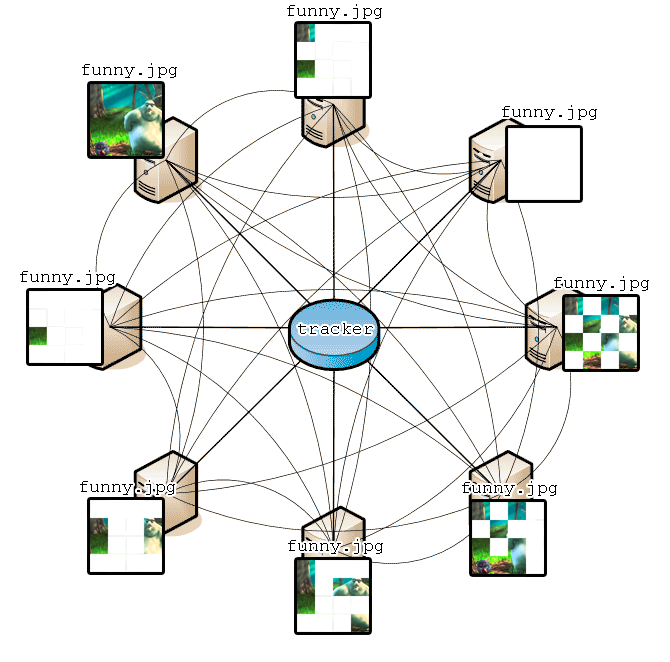
\includegraphics[width=10cm]{figuras/BITTORRENT_02}}
		}{
			\Fonte{Extraída de \citeonline{johnsen2005peer} e adaptada pelo autor}
		}
	\end{figure}

A Figura~\ref{fig:bittorrent-2}  mattis placerat risus sit amet laoreet. Praesent sapien arcu, maximus ac fringilla efficitur, vulputate faucibus sem. Donec aliquet velit eros, sit amet elementum dolor pharetra eget. Integer eget mattis libero na

\section{Fundamentação Teórica B}
\label{sec:fundamentacao-teorica-b}

Integer non lacinia magna. Aenean tempor lorem tellus, non sodales nisl commodo ut. Proin mattis placerat risus sit amet laoreet. Praesent sapien arcu, maximus ac fringilla efficitur, vulputate faucibus sem. Donec aliquet velit eros, sit amet elementum dolor pharetra eget. Integer eget mattis libero. Praesent ex velit, pulvinar at massa vel, fermentum dictum mauris. Ut feugiat accumsan

Nunc ac pretium dui. Mauris aliquam dapibus nulla ac mattis. Aenean non tortor volutpat, varius lectus vitae, accumsan nibh. Cras pretium vestibulum enim, id ullamcorper tortor ultrices non. Integer sodales viverra faucibus. Curabitur at dui lacinia, rhoncus lacus at, blandit metus. Integer scelerisque non enim quis ornare.

	\begin{table}[h!]
		\centering
		\Caption{\label{tab:end-privados} Intervalos de endereços privados reservados}
		\UFERSAtab{}{
			\begin{tabular}{lll}
				\toprule
				\multicolumn{2}{c}{Intervalo}&\\
				Limite inferior & Limite superior & Quantidade de hosts \\
				\midrule \midrule
				10.0.0.0	& 10.255.255.255	& 16.777.216 hosts\\
				172.16.0.0	& 172.31.255.255	& 1.048.576 hosts\\
				192.168.0.0	& 192.168.255.255	& 65.536 hosts\\
				\bottomrule
			\end{tabular}
		}{
			\Fonte{Adaptação extraída de \citeonline{rekhter1996address}}
		}
	\end{table}

Duis faucibus, enim quis tincidunt pellentesque, nisl leo varius nulla, vitae tempus dui mauris ac ante. Quisque purus lorem, pharetra sit amet lobortis eu, vehicula vitae purus.

Duis faucibus, enim quis tincidunt pellentesque, nisl leo varius nulla, vitae tempus dui mauris ac ante. Quisque purus lorem, pharetra sit amet lobortis eu, vehicula vitae purus: \acrlong{Bel}, \acrlong{Dr}, \acrlong{Esp}, \acrlong{GE}, \acrlong{GI}, \acrlong{IES}, \acrlong{Me}, \acrlong{SBGC}, \acrlong{UI}.

Duis faucibus, enim quis tincidunt pellentesque, nisl leo varius nulla, vitae tempus dui mauris ac ante. Quisque purus lorem, pharetra sit amet lobortis eu, vehicula vitae purus. Ut varius, erat nec vehicula elementum, risus est tempus justo, conforme ilustrado na Figura~\ref{fig:tanebaum-nat}.

\begin{figure}[h!]
	\centering
	\Caption{\label{fig:tanebaum-nat} Posicionamento e operação de um NAT}
	\UFERSAfig{}{
		\fbox{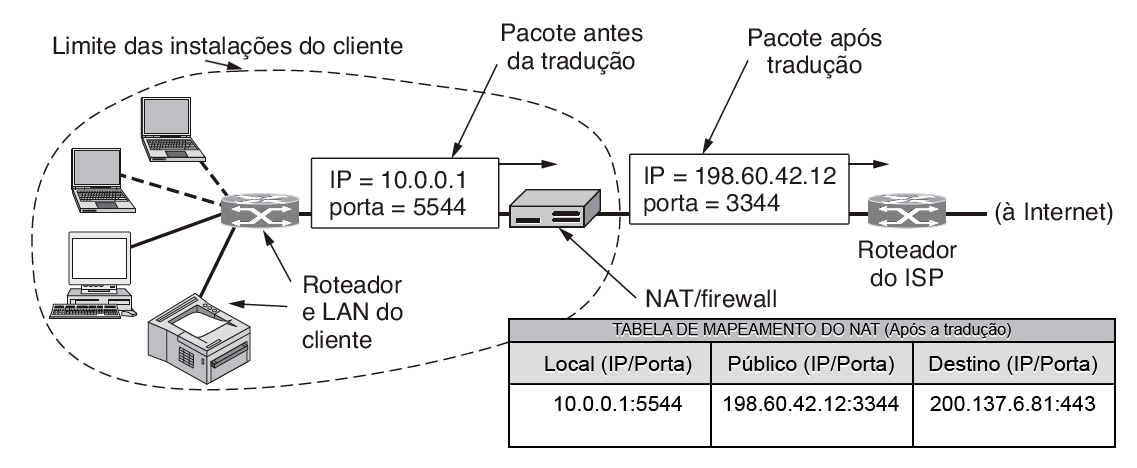
\includegraphics[width=13cm]{figuras/TANENBAUM_NAT_1}}
	}{
		\Fonte{Extraída de \citeonline{wetherall2011redes} alterado pelo autor}
	}
\end{figure}
